\section{Domäne}

Das nachfolgende Domänen-Modell (Abbildung \ref{fig:domainmodel}) zeigt alle nötigen Attribute für die Umsetzung der Applikation. Es beinhaltet die von den Agents erhaltenen Daten (grün), die konfigurierbaren Daten, wie beispielsweise Benutzer, Rollen und Gruppenzugehörigkeiten (rot) und ausserdem die Informationen, welche für die Auftragsverwaltung benötigt werden (gelb).

\begin{figure}
  \centering
    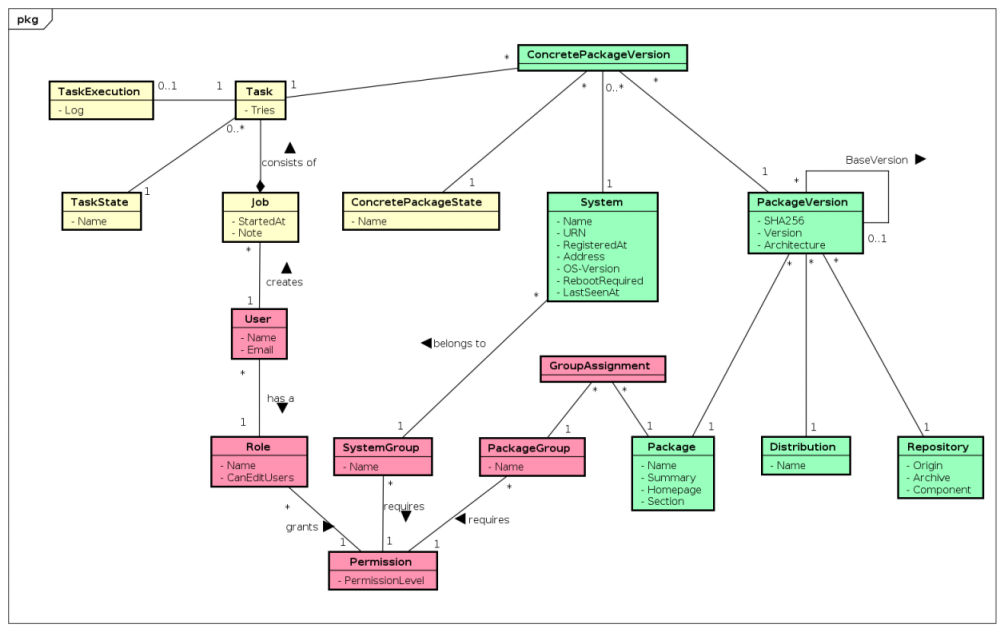
\includegraphics[width=\textwidth]{files/DomainModel_small}
  \caption{Domänen-Modell}
  \label{fig:domainmodel}
\end{figure}

\subsection*{Erläuterungen}

\subsubsection{System}

Ein System repräsentiert einen einzelnen Server, auf welchem die Updates verwaltet werden sollen. Relevante Daten über die Systeme werden erfasst oder beim Registrieren durch den Agent mitgeteilt.

\subsubsection{Package}

Ein Package ist ein einzelnes Applikationspaket, welches vom Paketmanager (hier: \gls{apt}) verwaltet wird. Beispiele dafür sind vim, openssl oder sudo. Das Paket selbst ist unabhängig von Versionen oder Distributionen.

\subsubsection{PackageVersion}

Eine Paket-Version ist eine verfügbare Version eines bestimmten Paketes auf einem spezifischen Repository/einer Distribution. Eine spezifische Paket-Version kann eine Base-Version sein. Das bedeutet, dass diese Paket-Version zusammen mit der Distribution ausgeliefert wurde. Wenn eine Paket-Version keine Base-Version ist, kann sie aber einen optionalen Verweis auf eine frühere Version besitzen.

\subsubsection{ConcretePackageVersion}

Eine Paket-Version kann mit einem System in Verbindung gebracht werden, zum Beispiel indem der Agent eine bestimmte Paket-Version als ausstehendes Update meldet. Diese Verbindung ist eine konkrete Paket-Version und zeigt, welchen Zustand diese Version auf diesem Paket hat (definiert durch einen \textbf{ConcretePackageState}):

\begin{itemize}
    \item Installiert
    \item Veraltet
    \item Ausstehend
    \item Fehlgeschlagen
    \item In Auftrag gegeben
\end{itemize}


\subsubsection{Distribution}

Eine Distribution, oft auch 'Distro' genannt, ist ein Betriebssystem basierend auf dem Linux-Kernel. Beispiele: Debian, Suse oder Ubuntu. Diese werden wiederum in spezifische Distros unterteilt, etwa bei Ubuntu auf Ubuntu 12.04 precise, 14.04 trusty oder 16.04 xenial.

\subsubsection{Repository}

Ein Repository ist eine Sammlung von Paketen für eine bestimmte Distribution.

\subsubsection{Job}

Ein Job wird dann erstellt, wenn ein Benutzer einen Auftrag erteilt. Pro betroffenem System enthält dieser Job einen Task, welcher dann an die Agenten geschickt wird.

\subsubsection{Task}

Ein Task enthält alle konkreten Aufträge für ein spezifisches System, welche von einem User in einem Durchgang erfasst wurden. Ein Task kann sich in den folgenden Zuständen (\textbf{TaskState}) befinden:

\begin{itemize}
    \item Erledigt 
    \item Fehlgeschlagen 
    \item Ausstehend
    \item In Bearbeitung
    \item Nicht zugestellt
\end{itemize}

Ein Task kann eine \textbf{TaskExecution} beinhalten, welche bei der Rückmeldung vom Agent mitgeliefert wird. Sie enthält lediglich die Ausgabe von \gls{apt}, welches vom Agent direkt weitergeschickt wird.

\subsubsection{User}

Ein User ist ein Benutzer, welcher sich über seine Email-Adresse und sein Passwort identifiziert und einen Namen und eine Rolle (\textbf{Role}) besitzt.

\subsubsection{Role}

Eine Rolle definiert, zu welcher Gruppe ein Benutzer gehört und welche Rechte dieser besitzt. Einerseits wird definiert, ob andere Benutzer bearbeitet werden können, andererseits wird ein \textbf{PermissionLevel} zugewiesen.

\subsubsection{PermissionLevel} \label{sec:domain:permission_level}

Paketgruppen, Systemgruppen sowie Rollen besitzen alle ein PermissionLevel. Diese Zahl bestimmt, ob ein Benutzer mit einer bestimmten Rolle das Recht besitzt, Systeme oder Pakete in spezifischen Gruppen zu bearbeiten und zu aktualisieren. Dazu muss das PermissionLevel der Rolle des Benutzers höher sein als das benötigte PermissionLevel der Gruppe des Systems.

Bei Paketen, welche in mehreren Gruppen sein können (über ein \textbf{GroupAssignment}), gilt das höchste PermissionLevel.